\chapter{Espín, isoespín, color e interacción propia de los gluones}

\section{Cromodinámica cuántica por analogía con la electrodinámica}

La cromodinámica cuántica es un tema demasiado amplio para desarrollarlo por completo en una sola lección. Aquí se busca presentar la imagen intuitiva básica, no profundizar en las matemáticas.

La electrodinámica cuántica es la teoría de los electrones y los fotones. También es la teoría cuántica de la fuerza de Coulomb. Si se trata el núcleo de un átomo como una fuente fija de campo eléctrico, sin considerar su movimiento ni su estructura interna, la QED es la teoría del átomo.

La cromodinámica cuántica desempeña un papel análogo para los quarks y los gluones. Describe las partículas mismas, las fuerzas entre ellas y los objetos compuestos que forman. Estos compuestos se llaman \emph{hadrones}. Los protones y los neutrones son bariones: tienen un número neto de quarks o, de manera equivalente, un número bariónico distinto de cero. Los mesones son combinaciones de quark--antiquark. Tanto los bariones como los mesones también contienen gluones.

Los gluones son eléctricamente neutros, pero proporcionan el campo que liga los quarks. En ese sentido, el campo de gluones cumple una función análoga a la del campo electromagnético que liga los átomos.

Antes de introducir el color y los gluones, conviene volver a las matemáticas del espín. Las mismas matemáticas reaparecen casi directamente como \emph{isospín}, y un patrón relacionado vuelve a aparecer en la teoría del color. La teoría de grupos subyace a estas construcciones, pero las ideas necesarias pueden desarrollarse a partir del momento angular.

\section{Multipletes de momento angular}

Las componentes del momento angular obedecen
\begin{equation}
[L_x,L_y]=i\hbar L_z,
\end{equation}
con las relaciones cíclicas correspondientes
\begin{equation}
[L_y,L_z]=i\hbar L_x,
\qquad
[L_z,L_x]=i\hbar L_y.
\end{equation}
Las tres componentes no conmutan, así que no pueden medirse todas simultáneamente. Por ello, una descripción elige un eje, convencionalmente el eje \(z\), y etiqueta los estados según la componente del momento angular a lo largo de ese eje.

Esta elección no rompe la simetría rotacional de la naturaleza. Solo rompe la simetría de la descripción, al elegir una dirección como referencia para organizar los estados.

Los valores permitidos de la componente \(z\) están cuantizados y difieren en una unidad de \(\hbar\). Al fijar \(\hbar=1\) para enumerar estos valores, un multiplete de espín \(\ell\) contiene
\begin{equation}
m=\ell,\ell-1,\ldots,-\ell.
\end{equation}
Por tanto, el número de estados independientes es
\begin{equation}
2\ell+1.
\end{equation}

Conviene escribir explícitamente los primeros multipletes:
\begin{align}
\ell=0:&\qquad m=0,\\
\ell=\frac12:&\qquad m=\frac12,-\frac12,\\
\ell=1:&\qquad m=1,0,-1,\\
\ell=\frac32:&\qquad
m=\frac32,\frac12,-\frac12,-\frac32,\\
\ell=2:&\qquad m=2,1,0,-1,-2.
\end{align}

Para nuestros propósitos, el espín semientero corresponde a los fermiones y el espín entero, a los bosones. El electrón es una partícula de espín \(\tfrac12\). Una partícula de espín cero no tiene momento angular en absoluto. El fotón tiene espín uno, y también hay estados de espín uno en átomos y núcleos. Los átomos y los núcleos también pueden tener espín \(\tfrac32\), y el mismo recuento continúa para espines mayores.

La notación debe distinguir el espín total de su componente. El número \(\ell\) etiqueta el multiplete y también es el valor máximo posible de la componente \(z\). El número \(m\) etiqueta un estado particular dentro de ese multiplete. Así, un objeto de espín uno tiene tres estados, mientras que uno de espín \(\tfrac12\) tiene dos.

\section{Combinación de dos partículas de espín un medio}

Consideremos dos partículas de espín \(\tfrac12\) e ignoremos su momento angular orbital. Su espacio producto de espín contiene cuatro estados de base:
\begin{equation}
|\uparrow\uparrow\rangle,\qquad
|\uparrow\downarrow\rangle,\qquad
|\downarrow\uparrow\rangle,\qquad
|\downarrow\downarrow\rangle.
\end{equation}
Las componentes \(z\) correspondientes son
\begin{align}
|\uparrow\uparrow\rangle &: m=+1,\\
|\uparrow\downarrow\rangle &: m=0,\\
|\downarrow\uparrow\rangle &: m=0,\\
|\downarrow\downarrow\rangle &: m=-1.
\end{align}

El estado en que ambos espines apuntan hacia arriba demuestra que debe haber un multiplete de espín uno: la componente \(z\) máxima es \(+1\). Un multiplete de espín uno tiene solo tres estados,
\begin{equation}
m=+1,\quad 0,\quad -1.
\end{equation}
Pero el espacio producto contiene cuatro estados, incluidos dos estados independientes con \(m=0\). No todos pueden pertenecer a un solo multiplete de espín uno. El estado restante no puede tener espín dos, porque un multiplete de espín dos requeriría cinco estados. Por tanto, los cuatro estados producto deben repartirse en tres estados de espín uno y un estado de espín cero.

¿Qué combinación de los dos estados de base \(m=0\) pertenece al multiplete de espín uno? Intercambiemos las dos partículas. Los estados alineados no cambian:
\begin{equation}
|\uparrow\uparrow\rangle\longrightarrow|\uparrow\uparrow\rangle,
\qquad
|\downarrow\downarrow\rangle\longrightarrow|\downarrow\downarrow\rangle.
\end{equation}
En cambio, los estados producto mixtos se intercambian:
\begin{equation}
|\uparrow\downarrow\rangle
\longleftrightarrow
|\downarrow\uparrow\rangle.
\end{equation}
La suma de ambos es simétrica bajo el intercambio:
\begin{equation}
|\uparrow\downarrow\rangle+|\downarrow\uparrow\rangle.
\end{equation}
La normalización introduce un factor de \(1/\sqrt2\):
\begin{equation}
|1,0\rangle
=
\frac{|\uparrow\downarrow\rangle
      +|\downarrow\uparrow\rangle}{\sqrt2}.
\end{equation}

\begin{figure}[h]
\centering
\includegraphics[width=0.78\textwidth]{lecture_02_figure_02.png}
\caption{Combinación mixta simétrica de espines que forma el miembro \(m=0\) del triplete de espín uno.}
\lectureframe{00:15:08}
\end{figure}

Junto con los dos estados alineados, esto da el triplete de espín uno:
\begin{align}
|1,+1\rangle &=|\uparrow\uparrow\rangle,\\
|1,0\rangle &=
\frac{|\uparrow\downarrow\rangle
      +|\downarrow\uparrow\rangle}{\sqrt2},\\
|1,-1\rangle &=|\downarrow\downarrow\rangle.
\end{align}
La combinación ortogonal restante lleva un signo menos:
\begin{equation}
|0,0\rangle
=
\frac{|\uparrow\downarrow\rangle
      -|\downarrow\uparrow\rangle}{\sqrt2}.
\end{equation}
Es antisimétrica bajo el intercambio y forma el multiplete de un solo estado con espín cero. Así,
\begin{equation}
\frac12\otimes\frac12=1\oplus0.
\end{equation}

El estado mixto simétrico tiene \(m=0\), pero \emph{no} tiene momento angular total cero. Pertenece al triplete de espín uno. Al rotar el eje de coordenadas, se mezcla con los estados \(m=\pm1\). Solo la combinación antisimétrica tiene \(\ell=0\).

En lo que respecta al momento angular, el singlete es como el espacio vacío. Puede tener energía, carga u otros números cuánticos, pero no tiene momento angular.

Esta distinción puede comprobarse mediante un experimento mental. Ignorando todas las leyes de conservación salvo la del momento angular, preguntemos qué estado de espín de dos partículas podría desaparecer sin más. Ninguno de los estados alineados podría desaparecer, porque ambos pertenecen a un multiplete de espín uno. Tampoco podría desaparecer el estado simétrico \(m=0\). Aunque su componente \(z\) se anula, su espín total sigue siendo uno, con componentes no triviales respecto de otros ejes. Solo el singlete antisimétrico podría desaparecer sin violar la conservación del momento angular.

\begin{classroomqa}
\audiencequestion{¿Una medición del estado mixto simétrico a lo largo del eje \(z\) daría \(+1\) o \(-1\)?\lecturetimestamp{00:19:28}}
\lecturerresponse{No. A lo largo del eje \(z\) da cero. Sin embargo, el estado tiene espín total uno, así que una medición a lo largo de otro eje puede dar \(+1\) o \(-1\).}
\end{classroomqa}

\section{Tres partículas de espín un medio}

Combinemos ahora tres partículas de espín \(\tfrac12\). Hay
\begin{equation}
2\times2\times2=8
\end{equation}
estados producto. Si los tres espines apuntan hacia arriba, la componente \(z\) total es \(+\tfrac32\). Por tanto, debe haber un multiplete de espín \(\tfrac32\). Contiene
\begin{equation}
2\left(\frac32\right)+1=4
\end{equation}
estados.

Quedan cuatro estados. No pueden formar un segundo multiplete de espín \(\tfrac32\), porque los estados con \(m=\pm\tfrac32\) ya se han utilizado. Los estados restantes tienen como componentes máximas solo \(+\tfrac12\) y \(-\tfrac12\). Tampoco pueden tres espines semienteros dar un espín total cero. Por tanto, los estados restantes deben formar multipletes de espín \(\tfrac12\).

Un multiplete de espín \(\tfrac12\) contiene dos estados. Como quedan cuatro estados, hay dos multipletes distintos de espín \(\tfrac12\):
\begin{equation}
\frac12\otimes\frac12\otimes\frac12
=
\frac32\oplus\frac12\oplus\frac12.
\end{equation}
Este patrón reaparecerá cuando los dos estados llamados espín hacia arriba y espín hacia abajo se sustituyan por los dos sabores de quark llamados arriba y abajo.

\section{El isospín como espín interno}

El isospín, o espín isotópico, es un análogo interno del espín ordinario. El espín ordinario está ligado a las rotaciones del espacio físico; el isospín, no. Se refiere a transformaciones en un espacio matemático interno, cuyos dos estados básicos se identificarán con
\begin{equation}
u,\qquad d.
\end{equation}
Aquí, los términos \emph{arriba} y \emph{abajo} son meras etiquetas de sabor. Nada apunta hacia arriba o hacia abajo en el espacio ordinario.

\editorialnote{No es posible recuperar con seguridad una breve transición entre la definición del espacio de espín interno y el argumento siguiente sobre la escala de masas hadrónicas. No se infiere de ella ninguna afirmación física adicional.}

¿Por qué \(u\) y \(d\) son adecuados para esta analogía? La escala de energía natural de la física de hadrones es de unos cientos de MeV. Un mesón ligero típico tiene una masa de unos cientos de MeV, y la energía implicada en ligar tres quarks para formar un nucleón está en esa misma escala. En comparación, las energías de enlace de los núcleos ordinarios son de apenas unos pocos MeV. Así pues, la fuerza que mantiene unidos a protones y neutrones dentro de un núcleo se considera en una escala de energía mucho menor que la de la dinámica que liga los quarks dentro de un hadrón.

Entre los seis sabores de quark, \(u\) y \(d\) son ligeros en comparación con la escala hadrónica. Producir quarks pesados requiere más energía, y los hadrones que los contienen pueden decaer en hadrones más ligeros. En consecuencia, los hadrones ligeros más estables están formados por quarks arriba y abajo.

El quark abajo es más pesado que el quark arriba, aproximadamente por un factor de dos según las estimaciones empleadas aquí, pero las masas de ambos son pequeñas en comparación con cientos de MeV. En primera aproximación, se pueden tratar a ambos como casi sin masa en la escala hadrónica. Más importante aún, se pueden tratar como si tuvieran masas casi iguales.

Esta igualdad aproximada da lugar a una simetría. Si se intercambian los quarks arriba y abajo, la física de la interacción fuerte cambia muy poco. El protón,
\begin{equation}
p\sim uud,
\end{equation}
y el neutrón,
\begin{equation}
n\sim udd,
\end{equation}
son el ejemplo más sencillo: difieren en el intercambio de \(u\) y \(d\), y sus masas son muy parecidas.

Por tanto, el intercambio
\begin{equation}
u\longleftrightarrow d
\end{equation}
se trata matemáticamente de manera análoga a
\begin{equation}
|\uparrow\rangle\longleftrightarrow|\downarrow\rangle.
\end{equation}
Para el espín ordinario, la transformación corresponde a una rotación de un eje en el espacio. Para el isospín, es una rotación en un espacio interno. Las matemáticas son análogas, aunque los significados físicos sean distintos.

\begin{figure}[h]
\centering
\includegraphics[width=0.80\textwidth]{lecture_02_figure_03.png}
\caption{Descomposición en triplete y singlete de dos estados de espín \(\tfrac12\), modelo de la construcción correspondiente para el isospín.}
\lectureframe{00:27:42}
\end{figure}

El prefijo \emph{iso} proviene de \emph{isótopo}. En la descripción nuclear antigua, se consideraba al protón y al neutrón como dos miembros de un mismo doblete interno. Intercambiar un protón y un neutrón en un núcleo transforma un isótopo en otro. Más tarde, el modelo de quarks atribuyó este intercambio entre protón y neutrón al intercambio subyacente de \(u\) y \(d\).

\begin{classroomqa}
\audiencequestion{¿El isospín existía antes que el modelo de quarks?\lecturetimestamp{00:30:19}}
\lecturerresponse{Sí. El isospín se introdujo antes que los quarks y se asocia históricamente con Heisenberg. Más tarde, el modelo de quarks proporcionó su interpretación en términos de los sabores \(u\) y \(d\).}
\end{classroomqa}

El isospín no es una simetría exacta de la naturaleza. Las masas de los quarks arriba y abajo no son exactamente iguales y sus cargas eléctricas son distintas:
\begin{equation}
Q(u)=+\frac23,
\qquad
Q(d)=-\frac13.
\end{equation}
Incluso si sus masas fueran iguales, el electromagnetismo seguiría distinguiéndolos.

En sistemas hadrónicos y nucleares pequeños, los efectos electromagnéticos son débiles en comparación con la interacción fuerte. En un núcleo grande, la repulsión eléctrica puede ser importante; para un protón, un neutrón o un núcleo pequeño como el helio, es una corrección relativamente pequeña en comparación con la escala de la interacción fuerte. Por tanto, la aproximación de isospín consta de dos pasos:

\begin{enumerate}
\item despreciar la diferencia de masas entre \(u\)--\(d\);
\item anular su distinción electromagnética y conservar solo la interacción fuerte.
\end{enumerate}

Dentro de esta aproximación, la transformación entre \(u\) y \(d\) se convierte en una simetría matemáticamente análoga a la simetría del espín ordinario.

\section{El doblete de isospín del nucleón}

No se puede aislar un quark individual para examinarlo como objeto libre en el laboratorio. Los bariones observados más sencillos contienen tres quarks. Por tanto, el argumento de recuento para tres espines tiene un análogo directo para el isospín: tres quarks con isospín \(\tfrac12\) pueden formar un isospín total \(\tfrac32\) o \(\tfrac12\).

Empecemos por el isospín total \(\tfrac12\). Tal multiplete tiene
\begin{equation}
2\left(\frac12\right)+1=2
\end{equation}
estados. Son el protón y el neutrón:
\begin{equation}
p\sim uud,
\qquad
n\sim udd.
\end{equation}
Sus cargas son
\begin{align}
Q(p)
&=\frac23+\frac23-\frac13
=+1,\\
Q(n)
&=\frac23-\frac13-\frac13
=0.
\end{align}
El intercambio de \(u\) y \(d\) intercambia el protón y el neutrón. Forman un doblete de isospín \(\tfrac12\).

Para hablar de simetría de intercambio, etiquetemos temporalmente las tres posiciones de quark con \(1,2,3\). No hay que confundir estas etiquetas con posiciones fijas de los quarks: estos se mueven. Un factor esquemático del protón es
\begin{equation}
d_1\bigl(u_2u_3-u_3u_2\bigr).
\end{equation}

\begin{figure}[h]
\centering
\includegraphics[width=0.58\textwidth]{lecture_02_figure_04.png}
\caption{Factor antisimetrizado de dos quarks \(u\) en un estado esquemático del protón.}
\lectureframe{00:35:43}
\end{figure}

La expresión busca destacar la antisimetría de intercambio fermiónica. No es la función de onda completa del protón. El estado completo debe combinar el sabor, el espín ordinario, la dependencia espacial y---, como pronto será esencial,---el color.

\editorialnote{Los subíndices son etiquetas temporales de posición o de partícula individual. Dos estados idénticos de sabor \(u\) no forman el singlete de isospín antisimétrico habitual, así que el factor mostrado por sí solo no permite concluir que el isospín sea cero. Se conserva únicamente como un paso local de antisimetrización de posiciones; el isospín total del protón se deduce de su estado completo de tres quarks.}

La comparación limitada con la construcción anterior del espín es que los estados cuánticos pueden combinarse de manera simétrica o antisimétrica bajo un intercambio de etiquetas. Esa comparación, por sí sola, no determina el isospín que lleva el factor \(uu\) mostrado.

El protón tiene espín ordinario \(\tfrac12\) e isospín \(\tfrac12\). Lo mismo ocurre con el neutrón. Son números cuánticos distintos: el espín ordinario se refiere a las rotaciones físicas, mientras que el isospín se refiere a la simetría interna \(u\)--\(d\).

\section{El cuarteto Delta}

Tres quarks ligeros también pueden formar un isospín total \(\tfrac32\). El multiplete resultante de cuatro estados es el cuarteto Delta:
\begin{equation}
\begin{aligned}
\Delta^{++}&\sim uuu,
&
\Delta^{+}&\sim uud,
\\
\Delta^{0}&\sim udd,
&
\Delta^{-}&\sim ddd.
\end{aligned}
\end{equation}
Los estados Delta tienen espín ordinario \(\tfrac32\), además de isospín \(\tfrac32\). En los estados con componentes máximas, los tres espines ordinarios están alineados, al igual que los tres isospines.

Una composición como \(uud\) no determina por sí sola si el estado es un protón o una \(\Delta^+\). El mismo contenido de sabor puede combinarse para dar estados con distintos espines e isospines totales.

\begin{classroomqa}
\audiencequestion{¿Qué distingue al miembro \(uud\) del cuarteto Delta de un protón?\lecturetimestamp{00:41:08}}
\lecturerresponse{Sus espines ordinarios son distintos. El protón tiene espín \(\tfrac12\), mientras que el estado Delta tiene espín \(\tfrac32\). Los quarks también están combinados en estados de isospín total distintos.}
\end{classroomqa}

\begin{classroomqa}
\audiencequestion{¿Son estados de isospín \(\tfrac12\) los miembros centrales del cuarteto Delta?\lecturetimestamp{00:41:52}}
\lecturerresponse{No. Sus componentes de isospín son \(+\tfrac12\) y \(-\tfrac12\), pero su isospín total es \(\tfrac32\). Un multiplete con isospín total \(\tfrac32\) contiene necesariamente cuatro estados de componente.}
\end{classroomqa}

Las cuatro componentes de isospín corresponden a
\begin{equation}
I_3=\frac32,\frac12,-\frac12,-\frac32.
\end{equation}
Sus cargas eléctricas son
\begin{align}
Q(\Delta^{++})&=+2,\\
Q(\Delta^{+})&=+1,\\
Q(\Delta^{0})&=0,\\
Q(\Delta^{-})&=-1.
\end{align}
Las cargas de los dos estados centrales coinciden con las del protón y el neutrón, pero los estados siguen siendo distintos porque sus acoplamientos de espín e isospín difieren.

La simetría aproximada del isospín hace que las masas de los cuatro estados Delta sean casi iguales. La pequeña diferencia de masas \(u\)--\(d\) produce solo una pequeña separación entre las masas del cuarteto. La escala de masas común de los Delta es aproximadamente
\begin{equation}
m_\Delta\sim1200\,\mathrm{MeV},
\end{equation}
mientras que el protón y el neutrón tienen masas cercanas a
\begin{equation}
m_N\sim940\,\mathrm{MeV}.
\end{equation}

\subsection{Decaimiento de la \texorpdfstring{\(\Delta^{++}\)}{Delta++}}

Los estados Delta tienen masa suficiente para decaer en un nucleón y un pión. Consideremos
\begin{equation}
\Delta^{++}\sim uuu.
\end{equation}
Al separarse los constituyentes, puede producirse un par quark--antiquark. Si se intentara insertar \(u\bar u\), quedaría un barión de tres quarks \(u\) en el estado final, y ese canal permitido más ligero no sería posible con la energía disponible. En cambio, producir un par \(d\bar d\) permite que los constituyentes se reagrupen como
\begin{equation}
uuu+d\bar d
\longrightarrow
uud+u\bar d.
\end{equation}
Los dos compuestos finales son
\begin{equation}
uud=p,
\qquad
u\bar d=\pi^+,
\end{equation}
por tanto,
\begin{equation}
\Delta^{++}\longrightarrow p+\pi^+.
\end{equation}

\begin{figure}[h]
\centering
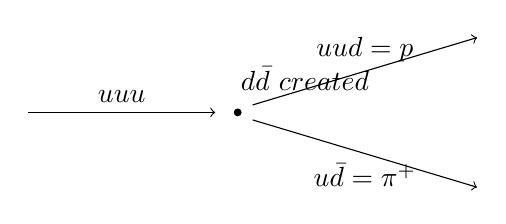
\begin{tikzpicture}[scale=0.95]
\draw[->] (-3,0) -- (-0.5,0) node[midway,above] {$uuu$};
\fill (-0.2,0) circle (1.5pt);
\draw[->] (0,0.1) -- (3,1.0) node[midway,above] {$uud=p$};
\draw[->] (0,-0.1) -- (3,-1.0) node[midway,below] {$u\bar d=\pi^+$};
\node at (0.7,0.45) {$d\bar d\ \text{created}$};
\end{tikzpicture}
\caption{Reagrupamiento de los constituyentes en el decaimiento \(\Delta^{++}\rightarrow p+\pi^+\).}
\end{figure}

La conservación de la carga es inmediata:
\begin{equation}
Q(p)+Q(\pi^+)=1+1=2=Q(\Delta^{++}).
\end{equation}
El balance aproximado de masas también permite el decaimiento:
\begin{equation}
1200\,\mathrm{MeV}
>
940\,\mathrm{MeV}+140\,\mathrm{MeV}.
\end{equation}
Queda energía suficiente para la energía cinética del estado final.

Los cuatro estados Delta pueden decaer en un protón o un neutrón junto con un pión. Sus tiempos de vida son extremadamente cortos. Se puede estimar su orden de magnitud con el tiempo que tarda la luz en cruzar un protón:
\begin{equation}
\tau_\Delta
\sim
\frac{10^{-13}\,\mathrm{cm}}
     {10^{10}\,\mathrm{cm/s}}
\sim10^{-23}\,\mathrm{s}.
\end{equation}
Aun así, viven lo suficiente para ser identificados como objetos distintos producidos en colisiones de partículas.

\begin{classroomqa}
\audiencequestion{En este recuento de constituyentes, ¿importa el orden escrito de los símbolos \(u\) y \(d\)?\lecturetimestamp{00:48:49}}
\lecturerresponse{Para lo que nos ocupa, no. Lo importante es el contenido de sabor y la manera de combinar el estado cuántico completo.}
\end{classroomqa}

\section{El problema de Pauli y la necesidad del color}

La \(\Delta^{++}\) plantea una contradicción. Está formada por tres quarks arriba. En un estado de espín \(\tfrac32\), sus espines ordinarios pueden apuntar todos en la misma dirección. Sus isospines también son idénticos, pues todos son \(u\). Si el espín, el sabor y el estado espacial de menor energía constituyeran toda la descripción, los tres quarks serían fermiones idénticos que ocupan el mismo estado. El principio de exclusión de Pauli lo prohíbe.

\begin{classroomqa}
\audiencequestion{¿Cómo pueden los quarks arriba repetidos ser fermiones si parecen ocupar el mismo estado?\lecturetimestamp{00:48:58}}
\lecturerresponse{No pueden ser idénticos en todos los números cuánticos. La \(\Delta^{++}\) muestra que los quarks necesitan una etiqueta adicional, además del espín ordinario, el sabor y el estado espacial. Esa etiqueta adicional es el color.}
\end{classroomqa}

La nueva etiqueta tiene tres valores posibles:
\begin{equation}
r,\qquad g,\qquad b,
\end{equation}
llamados rojo, verde y azul. Estas palabras no tienen nada que ver con los colores visibles. Son nombres arbitrarios para tres estados internos. Podrían haberse usado otros nombres; lo que importa es que haya tres posibilidades distintas.

Las versiones roja, verde y azul de un quark de un sabor dado tienen la misma masa y las mismas propiedades observables ordinarias. Sin embargo, son estados cuánticos distintos. Por tanto, una \(\Delta^{++}\) puede contener un \(u\) rojo, un \(u\) verde y un \(u\) azul, de modo que los tres fermiones no ocupan el mismo estado completo.

Los seis sabores son
\begin{equation}
u,\ d,\ c,\ s,\ t,\ b.
\end{equation}
Este orden no es por masa. El quark arriba es el más ligero y el quark abajo le sigue. El quark encanto es mucho más pesado que el quark extraño, y el quark cima es muchísimo más pesado que el quark fondo. Cada sabor se presenta en tres colores. Por tanto, un quark lleva al menos dos etiquetas internas distintas:
\begin{equation}
\text{flavor}\quad\text{and}\quad\text{color}.
\end{equation}

¿Podrían haberse distinguido los tres quarks por su posición o su momento? El problema Delta se refiere al estado de menor energía, en el que la estructura espacial y de momento pertinente no puede aportar tres etiquetas distintas sin cambiar la energía y las propiedades de simetría. La distinción que falta debe corresponder a un nuevo grado de libertad interno.

Hay una analogía ilustrativa con la función del espín en la física atómica. Dos electrones que parecen ocupar el mismo estado orbital aún pueden diferir en su estado de espín. De manera estructuralmente análoga, quarks que coinciden en sabor, espín ordinario y estado espacial pueden diferir en el color.

\editorialnote{Se indicó expresamente que era incierta la secuencia histórica precisa que vincula la espectroscopia del helio, el principio de Pauli y Uhlenbeck y Goudsmit. Se conserva la analogía sin afirmar que esta fuera la cronología exacta del descubrimiento del espín.}

Yoichiro Nambu está asociado con el reconocimiento de que los quarks necesitaban este grado de libertad adicional. El punto físico es independiente del nombre: tres colores de quark resuelven la contradicción de Pauli. El principio de exclusión pertinente es el principio de Pauli, no el principio de incertidumbre de Heisenberg.

\editorialnote{La atribución precisa y la historia posterior del nombre \emph{color} se dejaron como inciertas, así que aquí no se afirma una cronología más precisa. Se corrige una referencia oral al principio de incertidumbre de Heisenberg por el principio de exclusión de Pauli, como exige el argumento circundante sobre estadística fermiónica.}

La misma construcción del color se aplica al protón y al neutrón. Sus estados no se construyen asignando un color fijo y permanentemente identificable a cada símbolo de sabor escrito. Un barión físico es una superposición cuántica de las posibles asignaciones de rojo, verde y azul, combinadas con las simetrías de intercambio adecuadas.

\begin{classroomqa}
\audiencequestion{¿Es el color una propiedad física ordinaria que pueda medirse directamente?\lecturetimestamp{00:56:55}}
\lecturerresponse{Los tres colores tienen la misma masa y las mismas propiedades ordinarias. Su distinción se revela de manera relacional, mediante las combinaciones permitidas y los procesos de colisión. Los experimentos muestran que hay tres estados de color distintos, aunque no se pueda preparar un quark aislado con color para examinarlo directamente.}
\end{classroomqa}

\begin{classroomqa}
\audiencequestion{¿Se conserva el color?\lecturetimestamp{00:57:38}}
\lecturerresponse{Sí. El color se conserva, pero las partículas observables consideradas siempre tienen color cero, así que esta ley de conservación tiene un aspecto algo inusual.}
\end{classroomqa}

\editorialnote{Más precisamente, los hadrones asintóticos son singletes de color. La expresión ``color cero'' no designa una carga neta abeliana que se obtenga sumando numéricamente rojo, verde y azul.}

\begin{classroomqa}
\audiencequestion{¿Realmente necesita el protón \(uud\) por sí solo los tres colores? Parece bastar con distinguir los dos quarks \(u\).\lecturetimestamp{00:57:58}}
\lecturerresponse{Ese ejemplo requiere claramente alguna distinción adicional, pero no hace inevitable que haya tres. La \(\Delta^{++}\), con sus tres quarks arriba de espín ordinario paralelo e isospín paralelo, deja inequívocamente clara la necesidad de tres etiquetas distintas.}
\end{classroomqa}

Por eso la Delta desempeñó un papel tan importante. El protón y el neutrón tienen simetrías de espín y sabor más complicadas, así que los detalles de sus funciones de onda pueden ocultar la contradicción. En la \(\Delta^{++}\), el conflicto es inmediato:
\begin{equation}
uuu,\qquad
\uparrow\uparrow\uparrow,
\qquad
\text{one lowest spatial state}.
\end{equation}
Se requiere una nueva etiqueta con tres valores. Los datos de colisiones de hadrones confirman también de manera independiente la existencia de tres estados de color.

Una etiqueta de simetría puede tener significado aunque sus alternativas sean equivalentes cuando se consideran por separado. Sin un eje espacial elegido, dos direcciones de espín son físicamente equivalentes. Un segundo objeto puede proporcionar un eje de referencia y revelar la relación entre ambas. De manera similar, un protón o un neutrón selecciona una dirección en el espacio de isospín, y las comparaciones con otros estados revelan si las orientaciones internas son paralelas o antiparalelas. El color es más sutil, pero su contenido físico también se manifiesta mediante relaciones, correlaciones y reglas de interacción, no mediante colores visibles.

También se podría imaginar abandonar el principio de Pauli. Eso requeriría un marco matemático nuevo: la teoría cuántica de campos ordinaria clasifica las partículas como fermiones o bosones y no ofrece ninguna tercera opción establecida que resuelva este problema. La QCD conserva la naturaleza fermiónica de los quarks e introduce el color.

\begin{classroomqa}
\audiencequestion{¿Qué observable corresponde a la distinción oculta que exige el principio de Pauli?\lecturetimestamp{01:01:08}}
\lecturerresponse{Esa pregunta es mucho más sutil que las conocidas sobre posición, momento o isospín. Para responderla por completo hace falta conocer mejor la dinámica del color; lo dejamos para más adelante.}
\end{classroomqa}

\begin{classroomqa}
\audiencequestion{¿Se dedujo el carácter fermiónico de los quarks a partir de las asignaciones de espín de los hadrones?\lecturetimestamp{01:01:43}}
\lecturerresponse{Sí.}
\end{classroomqa}

\editorialnote{La formulación de las dos preguntas del público anteriores está parcialmente oscurecida. Se conocen con certeza sus temas y las respuestas breves, pero no se infiere una formulación más detallada.}

\begin{classroomqa}
\audiencequestion{¿Cómo se puede asociar un color particular a un quark del protón?\lecturetimestamp{01:01:55}}
\lecturerresponse{No se asigna un color fijo a un constituyente que pueda identificarse de manera permanente. El protón es una superposición cuántica de todas las asignaciones permitidas de rojo, verde y azul, con los factores de espín, sabor, espacio y color simetrizados o antisimetrizados según corresponda. La \(\Delta^{++}\) es útil porque su estructura de espín y sabor paralelos deja clara la necesidad del color sin exigir la función de onda completa del protón.}
\end{classroomqa}

El color desempeña en la QCD el papel que la carga eléctrica desempeña en la electrodinámica: es el número cuántico que controla la interacción. La QCD describe con gran precisión los datos experimentales de colisiones de hadrones. La justificación última del marco teórico es que sus consecuencias concuerdan con los experimentos.

\section{Fotones y gluones}

Los quarks son las partículas fermiónicas de materia de la QCD, análogas a los electrones de la QED en este aspecto limitado. ¿Qué los mantiene unidos?

En electrodinámica, un electrón es una fuente de campo electromagnético. En el lenguaje de las partículas, emite y absorbe fotones, y el intercambio de fotones produce fuerzas entre partículas cargadas. De manera análoga, un quark es una fuente del campo de gluones y puede emitir y absorber gluones.

Los gluones se parecen a los fotones en varios aspectos importantes. Son partículas sin masa de espín uno y tienen estados de polarización semejantes a los de los fotones. Su momento y su polarización son propiedades dinámicas ordinarias. La diferencia crucial es que los gluones llevan información de color y, por tanto, interactúan entre sí.

Los fotones no tienen carga eléctrica. En el nivel elemental de la QED, un fotón no emite otro fotón y dos haces de luz se atraviesan sin interactuar. Existen interacciones fotón-fotón de orden superior muy débiles que involucran lazos de electrones, pero son efectos secundarios, no un acoplamiento directo del fotón consigo mismo. En el espacio vacío, el vértice elemental de la QED consiste simplemente en que un electrón emita o absorba un fotón.

\begin{figure}[h]
\centering
\begin{tikzpicture}[scale=1.0]
\draw[->] (-2,-1) -- (0,0);
\draw[->] (0,0) -- (2,-1);
\draw[smooth] plot coordinates {
(0,0) (0.16,0.27) (0.32,0.23) (0.48,0.52)
(0.64,0.48) (0.80,0.77) (0.96,0.73)
(1.12,1.02) (1.28,0.98) (1.44,1.27)
(1.60,1.23) (1.76,1.52)
};
\node at (-1.25,-0.75) {$e^-$};
\node at (1.25,-0.75) {$e^-$};
\node at (1.95,1.62) {$\gamma$};
\fill (0,0) circle (1.5pt);
\end{tikzpicture}
\caption{Vértice elemental de la QED: un electrón emite o absorbe un fotón.}
\end{figure}

Al invertir el sentido de una línea fermiónica, la interpretación como electrón pasa a ser una interpretación como positrón. La emisión, la absorción y los procesos cruzados con positrones son distintas reorganizaciones de este mismo vértice.

Como recurso de contabilidad, podemos fingir que un fotón tiene algunas propiedades de un par electrón--positrón. El par es eléctricamente neutro, y los espines alineados de un electrón y un positrón pueden formar un espín total uno. Si una interacción externa aporta la energía y el momento necesarios, un fotón puede producir un par electrón--positrón. Esto no significa que un fotón esté literalmente formado por un electrón y un positrón. La imagen del par ficticio aporta poco a la propia QED, pero su análogo de color resulta útil en la QCD.

\section{Etiquetas de color--anticolor para los gluones}

Representemos los tres estados de color de un quark mediante una columna:
\begin{equation}
q=
\begin{pmatrix}
r\\
g\\
b
\end{pmatrix}.
\end{equation}
Representemos las etiquetas correspondientes del antiquark mediante una fila:
\begin{equation}
\bar q=
\begin{pmatrix}
\bar r&\bar g&\bar b
\end{pmatrix}.
\end{equation}

Un gluón no es un estado ligado de quark--antiquark. Sin embargo, su contabilidad de color se comporta como si llevara un color y un anticolor. Por tanto, las etiquetas posibles se pueden organizar así:
\begin{equation}
\begin{pmatrix}
r\bar r&r\bar g&r\bar b\\
g\bar r&g\bar g&g\bar b\\
b\bar r&b\bar g&b\bar b
\end{pmatrix}.
\end{equation}
A primera vista, esto da nueve combinaciones.

\begin{classroomqa}
\audiencequestion{¿Son indistinguibles las entradas diagonales de color--anticolor?\lecturetimestamp{01:13:37}}
\lecturerresponse{No exactamente. Las entradas diagonales son distintas; lo que ocurre es que su suma no constituye un estado cuántico independiente.}
\end{classroomqa}

En realidad, solo hay ocho estados independientes de gluón. Las tres etiquetas diagonales no son simplemente indistinguibles entre sí, pero la suma diagonal particular
\begin{equation}
r\bar r+g\bar g+b\bar b
\end{equation}
no constituye un gluón adicional independiente de la QCD. Dejaremos para más adelante la explicación profunda de esta reducción. Para los argumentos actuales sobre el flujo de color, resulta útil trabajar con las nueve etiquetas aparentes y recordar que falta una combinación diagonal.

\section{El vértice quark--gluón}

Un quark puede emitir un gluón y salir con el mismo color o con otro distinto. Si entra un quark de color \(a\) y sale uno de color \(b\), el gluón emitido lleva la etiqueta de contabilidad \(a\bar b\):
\begin{equation}
a\longrightarrow b+(a\bar b).
\end{equation}
Por ejemplo:
\begin{equation}
r\longrightarrow g+(r\bar g).
\end{equation}
La línea de color rojo continúa dentro del gluón, mientras que la línea verde prosigue por el quark saliente y se invierte para convertirse en una línea antigreen en el gluón.

El quark no tiene por qué cambiar de color. La misma regla también permite
\begin{equation}
r\longrightarrow r+(r\bar r),
\end{equation}
o bien
\begin{equation}
r\longrightarrow b+(r\bar b).
\end{equation}

\begin{figure}[h]
\centering
\begin{tikzpicture}[scale=1.0]
\draw[->] (-2,-0.8) -- (0,0) node[midway,above] {$r$};
\draw[->] (0,0) -- (2,0.9) node[midway,above] {$g$};
\draw[smooth] plot coordinates {
(0,0) (0.20,-0.23) (0.40,-0.17) (0.60,-0.46)
(0.80,-0.40) (1.00,-0.69) (1.20,-0.63)
(1.40,-0.92) (1.60,-0.86) (1.80,-1.15)
(2.00,-1.09)
};
\node at (2.35,-1.12) {$r\bar g$};
\fill (0,0) circle (1.5pt);
\end{tikzpicture}
\caption{Un quark rojo se convierte en verde al emitir un gluón \(r\bar g\).}
\end{figure}

Este es uno de los elementos constitutivos elementales de la QCD.

\begin{classroomqa}
\audiencequestion{¿Solo puede emitirse un gluón cuando el quark cambia de color?\lecturetimestamp{01:17:15}}
\lecturerresponse{No. El quark saliente puede tener el mismo color u otro distinto. En ambos casos, la etiqueta de color--anticolor del gluón mantiene continuas las líneas de color.}
\end{classroomqa}

\section{El vértice de tres gluones}

La QCD tiene otra interacción elemental sin análogo elemental en la QED: un gluón puede interactuar directamente con otros gluones.

Partamos de un gluón \(r\bar b\). En el lenguaje del flujo de color, puede desdoblarse así:
\begin{equation}
r\bar b
\longrightarrow
r\bar g+g\bar b.
\end{equation}
La línea roja continúa dentro de \(r\bar g\), la línea antiazul continúa dentro de \(g\bar b\), y el par verde-antiverde conecta los dos gluones salientes. Esto da lugar a un vértice de tres gluones.

\begin{figure}[h]
\centering
\begin{tikzpicture}[scale=1.0]
\draw[smooth] plot coordinates {
(-2,0) (-1.80,0.12) (-1.60,-0.02) (-1.40,0.12)
(-1.20,-0.02) (-1.00,0.12) (-0.80,-0.02)
(-0.60,0.12) (-0.40,-0.02) (-0.20,0.12) (0,0)
};
\draw[smooth] plot coordinates {
(0,0) (0.20,0.27) (0.40,0.21) (0.60,0.50)
(0.80,0.44) (1.00,0.73) (1.20,0.67)
(1.40,0.96) (1.60,0.90) (1.80,1.19) (2.00,1.13)
};
\draw[smooth] plot coordinates {
(0,0) (0.20,-0.27) (0.40,-0.21) (0.60,-0.50)
(0.80,-0.44) (1.00,-0.73) (1.20,-0.67)
(1.40,-0.96) (1.60,-0.90) (1.80,-1.19) (2.00,-1.13)
};
\node at (-2.45,0) {$r\bar b$};
\node at (2.45,1.18) {$r\bar g$};
\node at (2.45,-1.18) {$g\bar b$};
\fill (0,0) circle (1.5pt);
\end{tikzpicture}
\caption{Flujo de color en el vértice de tres gluones: \(r\bar b\rightarrow r\bar g+g\bar b\).}
\end{figure}

No hace falta memorizar todas las combinaciones permitidas. Basta con seguir cada línea de color en el diagrama. Cuando una línea fermiónica invierte su sentido temporal, hay que reinterpretarla como la línea de la antipartícula o del anticolor correspondiente.

\section{Intercambio de gluones y fuerzas}

El intercambio de gluones produce fuerzas, del mismo modo que el intercambio de fotones entre partículas cargadas produce fuerzas electromagnéticas.

Por ejemplo, un quark azul y un antiquark antiazul pueden intercambiar un gluón \(g\bar b\) y salir como un quark verde y un antiquark antiverde. Una asignación del flujo de color que satisface ambos vértices es\footnote{El cambio neto de color \(b+\bar b\longrightarrow g+\bar g\) es explícito, pero las etiquetas de color locales se corrigen varias veces. La etiqueta intercambiada \(g\bar b\) se reconstruye exigiendo que el flujo de color sea continuo en ambos vértices.}
\begin{equation}
b+\bar b
\longrightarrow
g+\bar g.
\end{equation}
En el vértice del antiquark,
\begin{equation}
\bar b\longrightarrow\bar g+(g\bar b),
\end{equation}
mientras que en el vértice del quark,
\begin{equation}
b+(g\bar b)\longrightarrow g.
\end{equation}
El gluón intercambiado lleva el cambio de color de una línea fermiónica a la otra.

\begin{figure}[h]
\centering
\begin{tikzpicture}[scale=1.0]
\draw[->] (-1.8,0) -- (-1.8,-1.8) node[midway,left] {$\bar b$};
\draw[->] (-1.8,1.8) -- (-1.8,0) node[midway,left] {$\bar g$};
\draw[->] (1.8,-1.8) -- (1.8,0) node[midway,right] {$b$};
\draw[->] (1.8,0) -- (1.8,1.8) node[midway,right] {$g$};
\draw[smooth] plot coordinates {
(-1.8,0) (-1.50,0.13) (-1.20,-0.03) (-0.90,0.13)
(-0.60,-0.03) (-0.30,0.13) (0,-0.03)
(0.30,0.13) (0.60,-0.03) (0.90,0.13)
(1.20,-0.03) (1.50,0.13) (1.8,0)
};
\node at (0,0.42) {$g\bar b$};
\fill (-1.8,0) circle (1.5pt);
\fill (1.8,0) circle (1.5pt);
\end{tikzpicture}
\caption{El intercambio de un gluón \(g\bar b\) convierte un par azul--antiazul en un par verde--antiverde; las flechas de los antiquarks apuntan en sentido opuesto al del aumento del tiempo.}
\end{figure}

La misma interacción permite fuerzas entre gluones. Una realización coherente es\footnote{La clase establece el intercambio de gluones entre gluones y la regla de seguir las líneas, pero las etiquetas locales del diagrama se revisan varias veces. La asignación mostrada es una realización coherente de la regla final, no una transcripción segura de cada etiqueta intermedia.}
\begin{equation}
(r\bar b)+(b\bar r)
\longrightarrow
(r\bar g)+(g\bar r),
\end{equation}
con un gluón \(g\bar b\) intercambiado entre los dos gluones externos:
\begin{align}
r\bar b&\longrightarrow r\bar g+g\bar b,\\
b\bar r+g\bar b&\longrightarrow g\bar r.
\end{align}

\begin{figure}[h]
\centering
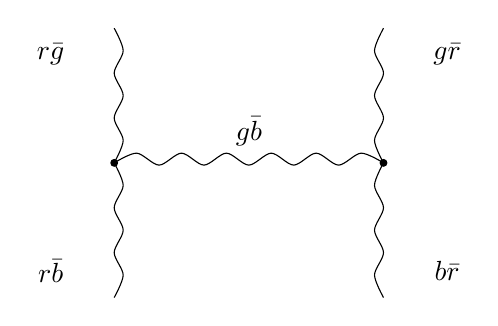
\begin{tikzpicture}[scale=0.95]
\draw[smooth] plot coordinates {
(-1.8,-1.8) (-1.68,-1.50) (-1.80,-1.20) (-1.68,-0.90)
(-1.80,-0.60) (-1.68,-0.30) (-1.8,0)
};
\draw[smooth] plot coordinates {
(-1.8,0) (-1.68,0.30) (-1.80,0.60) (-1.68,0.90)
(-1.80,1.20) (-1.68,1.50) (-1.8,1.8)
};
\draw[smooth] plot coordinates {
(1.8,-1.8) (1.68,-1.50) (1.80,-1.20) (1.68,-0.90)
(1.80,-0.60) (1.68,-0.30) (1.8,0)
};
\draw[smooth] plot coordinates {
(1.8,0) (1.68,0.30) (1.80,0.60) (1.68,0.90)
(1.80,1.20) (1.68,1.50) (1.8,1.8)
};
\draw[smooth] plot coordinates {
(-1.8,0) (-1.50,0.13) (-1.20,-0.03) (-0.90,0.13)
(-0.60,-0.03) (-0.30,0.13) (0,-0.03)
(0.30,0.13) (0.60,-0.03) (0.90,0.13)
(1.20,-0.03) (1.50,0.13) (1.8,0)
};
\node at (-2.65,-1.45) {$r\bar b$};
\node at (-2.65,1.45) {$r\bar g$};
\node at (2.65,-1.45) {$b\bar r$};
\node at (2.65,1.45) {$g\bar r$};
\node at (0,0.42) {$g\bar b$};
\fill (-1.8,0) circle (1.5pt);
\fill (1.8,0) circle (1.5pt);
\end{tikzpicture}
\caption{Intercambio de un gluón \(g\bar b\) entre dos gluones, con cada línea de color y anticolor continua a través de los vértices.}
\end{figure}

\section{Auto interacción de los gluones y campos no lineales}

La auto interacción de los gluones cambia el carácter de la QCD. Los quarks pueden unirse mediante el intercambio de gluones y formar hadrones, pero los gluones también pueden unirse mediante el intercambio de gluones. Por tanto, la QCD puede contener objetos compuestos íntegramente por grados de libertad gluónicos, sin quarks. En la QED no existe un estado ligado elemental correspondiente formado solo por fotones.

El lenguaje de campos lleva a la misma conclusión. En el nivel elemental, dos ondas electromagnéticas en el espacio vacío se atraviesan mutuamente. Dos ondas de gluones interactúan y se deforman entre sí. Incluso distintas partes de una misma configuración del campo de gluones pueden ejercer fuerzas unas sobre otras. Por tanto, el campo de gluones es no lineal.

\begin{classroomqa}
\audiencequestion{¿Deben aparecer las mismas cantidades de etiquetas roja, verde y azul a cada lado de un diagrama?\lecturetimestamp{01:24:59}}
\lecturerresponse{La regla práctica es seguir cada línea de color a través del diagrama. Esa continuidad es la conservación del color. Si una línea fermiónica invierte su sentido en el tiempo, su etiqueta pasa a ser la etiqueta correspondiente de antipartícula o de anticolor.}
\end{classroomqa}

\begin{classroomqa}
\audiencequestion{¿Son coherentes todas las etiquetas de color y anticolor de la primera versión del diagrama?\lecturetimestamp{01:26:00}}
\lecturerresponse{No. Hay que corregir varias etiquetas. En una asignación coherente, las líneas roja, antiazul y verde continúan cada una a través de los vértices; una flecha fermiónica invertida se interpreta como una antipartícula.}
\end{classroomqa}

\begin{classroomqa}
\audiencequestion{¿Se está tratando una línea de gluón intermedio como un par quark--antiquark?\lecturetimestamp{01:27:58}}
\lecturerresponse{Solo en la contabilidad de color. Un gluón no es literalmente un compuesto de quark--antiquark, pero lleva las propiedades correspondientes de color y anticolor.}
\end{classroomqa}

En esta etapa, las reglas elementales son concisas:

\begin{itemize}
\item los quarks emiten y absorben gluones;
\item los gluones interactúan directamente con otros gluones;
\item cada línea de color y anticolor debe continuar a través de un vértice;
\item al invertir una línea fermiónica en el tiempo, esta se convierte en la línea de la antipartícula correspondiente.
\end{itemize}

\begin{classroomqa}
\audiencequestion{¿Siguen siendo sin masa los gluones cuando se representan mediante todas estas líneas de color--anticolor?\lecturetimestamp{01:28:13}}
\lecturerresponse{Sí. Los gluones siguen siendo partículas sin masa. La precisión que viene a continuación se refiere al significado de la masa asignada a un quark dentro de un hadrón.}
\end{classroomqa}

A continuación vienen el confinamiento y la estructura de los hadrones: por qué nunca se observa color aislado y cómo se organizan los quarks y los gluones dentro de partículas compuestas. Primero conviene aclarar qué se entiende por la masa de un quark constituyente.

\section{Escala de sondeo y significado de la masa del quark}

Imaginemos un objeto pequeño de masa \(m\) unido a un trozo de material blando y deformable---; por ejemplo, un pedazo colgante de chicle. Apliquemos una fuerza muy suave y lentamente, para que el material blando tenga tiempo de ajustarse y todo el sistema se mueva en conjunto. La inercia medida será entonces la del objeto pequeño más la del material unido a él.

Ahora agitemos el objeto pequeño a una frecuencia muy alta. El material blando no tiene tiempo de acompañar el movimiento rápido. Permanece casi inmóvil mientras responde el núcleo pequeño. La inercia medida a alta frecuencia se aproxima entonces mucho más a la de \(m\) por sí solo.

\begin{figure}[h]
\centering
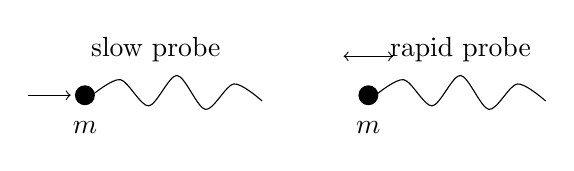
\begin{tikzpicture}[scale=0.9]
\fill (-3,0) circle (4pt);
\node at (-3,-0.45) {$m$};
\draw[smooth] plot coordinates {
(-2.9,0) (-2.5,0.22) (-2.1,-0.15) (-1.7,0.28)
(-1.3,-0.20) (-0.9,0.16) (-0.5,-0.08)
};
\draw[->] (-3.8,0) -- (-3.2,0);
\node at (-2.0,0.65) {slow probe};

\fill (1.0,0) circle (4pt);
\node at (1.0,-0.45) {$m$};
\draw[smooth] plot coordinates {
(1.1,0) (1.5,0.22) (1.9,-0.15) (2.3,0.28)
(2.7,-0.20) (3.1,0.16) (3.5,-0.08)
};
\draw[<->] (0.65,0.55) -- (1.35,0.55);
\node at (2.3,0.65) {rapid probe};
\end{tikzpicture}
\caption{Una sonda lenta mueve el núcleo y su acoplamiento blando en conjunto, mientras que una sonda rápida mide inicialmente sobre todo la respuesta del núcleo.}
\end{figure}

Esta es una analogía clásica. La masa inferida depende de la frecuencia de la fuerza aplicada, porque las distintas partes del sistema tienen tiempo para participar a frecuencias diferentes.

Un quark dentro de un hadrón está rodeado de material gluónico que interactúa fuertemente y de los demás constituyentes. Si se pudiera tirar muy lentamente de un quark, respondería el hadrón entero. La inercia encontrada sería entonces del orden de la masa del nucleón,
\begin{equation}
m_N\sim930\text{--}940\,\mathrm{MeV}.
\end{equation}
Si el quark recibe un golpe muy fuerte y se sondea durante un intervalo muy breve, la respuesta inicial corresponde al parámetro de masa mucho menor que se asigna convencionalmente a un quark ligero, aproximadamente
\begin{equation}
m_{u,d}\sim5\text{--}10\,\mathrm{MeV}
\end{equation}
en las estimaciones que usamos aquí.

Así pues, la expresión ``la masa de un quark''requiere especificar la escala de la sonda. Una perturbación suave y de baja frecuencia mueve el compuesto extendido; una perturbación intensa y de alta frecuencia permite resolver inicialmente una parte mucho menor. Esta analogía no es una derivación de la renormalización, pero ayuda a entender por qué los parámetros empleados para describir partículas dependen de las frecuencias y longitudes de onda de las interacciones en las que se miden. A estos parámetros dependientes de la escala se los llama parámetros corrientes o constantes corrientes.

\begin{classroomqa}
\audiencequestion{¿Es esta masa dependiente de la frecuencia simplemente otra forma de expresar una relación de incertidumbre como \(\Delta x\,\Delta t\)?\lecturetimestamp{01:33:32}}
\lecturerresponse{No. El ejemplo ya describe un fenómeno clásico. Una masa pequeña unida a algo blando acelera de una manera bajo una fuerza rápida y de otra bajo una fuerza lenta, porque distintas cantidades del material unido tienen tiempo para responder.}
\end{classroomqa}

\begin{classroomqa}
\audiencequestion{¿Tiene la discusión anterior de la carga eléctrica del electrón el mismo tipo de dependencia de escala?\lecturetimestamp{01:34:04}}
\lecturerresponse{Sí. La lección general es que los parámetros usados para describir partículas dependen de las frecuencias y longitudes de onda de las interacciones con las que se las sondea. Se llaman constantes corrientes.}
\end{classroomqa}

\begin{classroomqa}
\audiencequestion{¿Se aplica la misma precisión a la carga fraccionaria asignada a un quark?\lecturetimestamp{01:34:36}}
\lecturerresponse{Sí. Hay que definir cuidadosamente qué se entiende por la carga de un quark. En este nivel, se expresa en relación con la carga del protón; una definición más completa requiere una discusión aparte.}
\end{classroomqa}

\editorialnote{El número cuántico fijo de carga eléctrica fraccionaria y el acoplamiento de interacción dependiente de la escala son distintos. La evolución del acoplamiento no cambia las propias etiquetas de sabor \(+\tfrac23\) ni \(-\tfrac13\).}

\begin{classroomqa}
\audiencequestion{¿Por qué la contabilidad del color siempre usa un quark y un antiquark? ¿Por qué no podrían formar el objeto correspondiente dos quarks?\lecturetimestamp{01:34:55}}
\lecturerresponse{Es una pregunta importante, pero la respuesta corresponde a la siguiente discusión sobre las combinaciones de color permitidas y el confinamiento.}
\end{classroomqa}

\begin{classroomqa}
\audiencequestion{Si no se pueden aislar quarks individuales, ¿cómo se infirieron la carga fraccionaria, el color y el modelo de quarks?\lecturetimestamp{01:35:17}}
\lecturerresponse{La imagen fue surgiendo gradualmente a partir de muchas pistas y de aparentes contradicciones. Los patrones de los hadrones sugerían que estaban formados por quarks; los estados Delta revelaron un conflicto con la estadística de Fermi; y el confinamiento permanente de los quarks aportó otro hecho peculiar. La propuesta de los quarks apareció a principios de los 1960; Nambu presentó una versión temprana importante de la idea del color, y muchos físicos reunieron y pusieron a prueba la estructura completa a lo largo de aproximadamente la década siguiente. No fue resultado de una sola observación ni de una sola persona.}
\end{classroomqa}

\begin{classroomqa}
\audiencequestion{¿Por qué solo hay ocho gluones, en vez de las nueve combinaciones aparentes de color--anticolor?\lecturetimestamp{01:37:24}}
\lecturerresponse{Dejaremos para más adelante la explicación detallada de por qué la suma diagonal no es un gluón adicional.}
\end{classroomqa}

\begin{classroomqa}
\audiencequestion{¿Esta discusión de la QCD está dejando de lado los electrones?\lecturetimestamp{01:37:33}}
\lecturerresponse{Sí. Estamos aislando la QCD del mismo modo que una discusión de la QED puede dejar temporalmente de lado los quarks. A la larga, hay que combinar los sectores por separado en una estructura más amplia que incluya quarks, electrones, fotones y las demás partículas. Algunas partes de esa síntesis más amplia ya se han logrado y otras siguen incompletas. En física, a menudo se avanza aislando un subsistema, comprendiéndolo y luego volviendo a ensamblar las partes.}
\end{classroomqa}
